\section{Herbrand's Theorem}

\underline{1.} Find a standard form from for each of the following formulas:
\begin{itemize}
 \item[(a)] $ \sim ((\forall x) P(x) \implies (\exists y) (\forall z) Q(y,z)) $ \newline
$ P(x) \wedge \sim Q(y, f(x, y)) $
 \item[(b)] $ (\forall x)((\sim E(x,0)\implies((\exists y)(E(y,g(x)) \wedge (\forall z)(E(z,g(x)) \implies E(y,z))))) $ \newline
$ E(x,0) \vee (E(f(x),g(x)) \wedge ( (\sim E(z,g(x)) \vee E(f(x),z))) )$
 \item[(c)] $ \sim((\forall x)P(x) \implies(\exists y)P(y)) $.
 \newline
$ P(x) \vee P(f(x)) $
\end{itemize}

\underline{5.} Let S = \{P(f(x),a,g(f(x),b))\}.
\begin{itemize}
 \item[(1)] Find H0 and H1. \newline
$ H_0 = \{ a, b \} $ \newline
$ H_1 = \{ a, b, f(a), f(b), g(a, a), g(a, b), g(b, a), g(b, b) \} $
 \item[(2)] Find all the ground instances of S over H0. \newline
$ P(a), P(b), g(f(a)), g(f(b)) $
 \item[(3)] Find all the ground instances of S over H1. \newline
$ P(a), P(b), P(f(a)), P(f(b)), P(g(a,a)), P(g(a,b)), P(g(b,a)), P(g(b,b)),\\
g(f(a),b), g(f(b),b), g(f(f(a)),b), g(f(f(b)),b), g(f(g(a,a)),b),\\
g(f(g(a,b)),b),g(f(g(b,a)),b), g(f(g(b,b)),b)$
\end{itemize}

8. Consider the following clause C and interpreation I:

$ C: P(x) \vee Q(x,f(x)) $

$I:\\
\{ \sim P(a), \sim P(f(a)), \sim P(f(f(a))), ...,\\
\sim Q(a,a), Q(a, f(a)), \sim Q(a,f(f(a))), ...,\\
\sim Q(f(a,a),Q(f(a),f(a)), \sim Q(f(a), f(f(a))), ... \}.$

Does I satisfy C?

Não. S' = \{P(a), Q(a, f(a))\}.

\underline{9.} Consider the following set S of clauses:

\[
S =	\begin{cases}
		P(x) \\
		Q(f(y)).
	\end{cases}
\]

Let an interpretation I be defined as below:

$I =\\
\{P(a), P(f(a)), P(f(f(a))), ...,\\
Q(a), \sim Q(f(a)), Q(f(f(a))), ...\}.
$

Does I satisfy S?

Não. S' = \{P(a), Q(f(a))\}.

10. Consider $ S = \{P(x), \sim P(f(y))\} $.

\begin{itemize}
 \item[1.] Give H0, H1, H2, and H3 of S. \newline
$ H_0 = \{a\} $ \newline
$ H_1 = \{a, f(a)\} $ \newline
$ H_2 = \{a, f(a), f(f(a))\} $ \newline
$ H_3 = \{a, f(a), f(f(a)), f(f(f(a)))\} $
 \item[2.] Is it possible to find an interpreation that satisfies S? If yes, give one. If no, why?

Não existe interpretação que satisfaz S. Os dois primeiros termos da interpretação devem ser $I = \{ P(a), \sim P(f(a)) \}$. Considerando x = f(a), a fórmula já não seria satisfeita.
\end{itemize}

11. Let $ S = \{P, \sim P \vee Q, \sim Q\} $. Give a closed semantic tree of S.

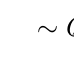
\begin{tikzpicture}[every tree node/.style={draw,circle},
   level distance=1.25cm,sibling distance=.5cm, 
   edge from parent path={(\tikzparentnode) -- (\tikzchildnode)}]
\Tree [.\node { };
        \edge node[left] {P};
        [.{ } 
          \edge node[left] {Q};
          [.{$ \square $} ]
          \edge node[right] {$\sim Q$};
          [.{$ \square $} ]
        ]
        \edge node[right] {$\sim P$};
        [.{$ \square $} ]
      ]
\end{tikzpicture}

12. Consider $ S = \{P(x), \sim P(x) \vee Q(x,a), \sim Q(y,a)\} $.
\begin{itemize}
 \item[(a)] Give the atom set of S. \newline
S = \{P(a), Q(a,a)\}
 \item[(b)] Give a complete semantic tree of S. \newline
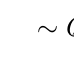
\begin{tikzpicture}[every tree node/.style={draw,circle},
   level distance=1.25cm,sibling distance=.5cm, 
   edge from parent path={(\tikzparentnode) -- (\tikzchildnode)}]
\Tree [.\node { };
        \edge node[left] {P(a)};
        [.{ } 
          \edge node[left] {Q(a,a)};
          [.{ } ]
          \edge node[right] {$\sim Q(a,a)$};
          [.{ } ]
        ]
        \edge node[right] {$\sim P(a)$};
        [.{ } 
          \edge node[left] {Q(a,a)};
          [.{ } ]
          \edge node[right] {$\sim Q(a,a)$};
          [.{ } ]
        ]
      ]
\end{tikzpicture}
 \item[(c)] Give a closed semantic tree of S. \newline
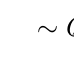
\begin{tikzpicture}[every tree node/.style={draw,circle},
   level distance=1.25cm,sibling distance=.5cm, 
   edge from parent path={(\tikzparentnode) -- (\tikzchildnode)}]
\Tree [.\node { };
        \edge node[left] {P(a)};
        [.{ }
          \edge node[left] {Q(a,a)};
          [.{$\square$} ]
          \edge node[right] {$\sim Q(a,a)$};
          [.{$\square$} ]
        ]
        \edge node[right] {$\sim P(a)$};
        [.{$\square$} ]
      ]
\end{tikzpicture}
\end{itemize}

13. Consider $ S = \{P(x,a,g(x,b)), \sim P(f(y),z,g(f(a),b))\} $. Find an unsatisfiable set S' of ground instances of clauses in S.

$ S' = \{ P(f(y),a,g(f(a),b)), \sim P(f(y),a,g(f(a),b)) \} $

\underline{14.} Let $ S = \{P(x),Q(x,f(x)) \vee \sim P(x), \sim Q(g(y),z)\} $. Find an unsatisfiable set S' of ground instances of clauses in S.

$ S' = \{ P(x), Q(g(y),f(g(y)))\vee \sim P(x), \sim Q(g(y),f(g(y)))\} $